\documentclass[a4paper]{article}

% --- UNIVERSAL PREAMBLE BLOCK ---
\usepackage[a4paper, top=1.5cm, bottom=1.5cm, left=1.5cm, right=1.5cm]{geometry}
\usepackage{fontspec}

\usepackage[indonesian, provide=*]{babel}
\babelprovide[import, onchar=ids fonts]{indonesian}
\babelprovide[import, onchar=ids fonts]{english}

% Set default/Latin font to Sans Serif (Noto Sans)
\babelfont{rm}{Noto Sans}
\babelfont{sf}{Noto Sans}

% Packages for graphics and layout
\usepackage{tikz}
\usetikzlibrary{shapes, shapes.symbols, arrows.meta, positioning, calc, shadows, backgrounds, patterns, decorations.pathreplacing}
\usepackage[most]{tcolorbox}
\usepackage{multicol}
\usepackage{enumitem}

% --- COLOR DEFINITIONS (MERGED) ---
% Colors from Part 1
\definecolor{mainBlue}{HTML}{2C3E50}
\definecolor{accentTeal}{HTML}{16A085}
\definecolor{softBgA}{HTML}{ECF0F1} % Renamed to distinguish
\definecolor{alertRed}{HTML}{E74C3C}
\definecolor{niceOrange}{HTML}{F39C12}
\definecolor{dotBlue}{HTML}{2980B9}
\definecolor{dotRed}{HTML}{C0392B}
\definecolor{lightPurple}{HTML}{9B59B6}

% Colors from Part 2 (Adding specific ones)
\definecolor{softBgB}{HTML}{F7F9F9} % Renamed to distinguish
\definecolor{powerBlue}{HTML}{2980B9}
\definecolor{solGreen}{HTML}{27AE60}

% --- SHARED CUSTOM COMMANDS ---
\newcommand{\checkbox}{\tikz[baseline=-0.6ex]{\draw[thick, mainBlue] (0,0) rectangle (0.3,0.3);}}

% Helper command to draw clean Ten Frame
% Usage: \DrawFrame{x_offset}{y_offset}
\newcommand{\DrawFrame}[2]{
    \draw[tfGrid, shift={(#1,#2)}] (0,0) grid (5,2);
    \draw[tfBorder, shift={(#1,#2)}] (0,0) rectangle (5,2);
}

% --- CUSTOM BOX FOR CASE STUDIES (PART 2) ---
\newtcolorbox{CaseStudyBox}[2][]{
    enhanced,
    colback=white,
    colframe=mainBlue!20!white,
    boxrule=0.5pt,
    left=2mm, right=2mm, top=2mm, bottom=2mm,
    title={\textbf{#2}},
    coltitle=mainBlue,
    fonttitle=\bfseries\large,
    attach boxed title to top left={yshift=-2mm, xshift=2mm},
    boxed title style={boxrule=0pt, colframe=white, colback=white},
    #1
}

\begin{document}

% =================================================================================
% PART 1: INTRODUCTION & CONTEXT
% =================================================================================

% --- TIKZ STYLES FOR PART 1 (Larger Scale) ---
\tikzset{
    tfPic/.style={x=0.7cm, y=0.7cm, baseline={([yshift=-.5ex]current bounding box.center)}},
    tfGrid/.style={draw=mainBlue, thin, step=1},
    tfBorder/.style={draw=mainBlue, very thick},
    counter/.style={circle, fill=dotBlue, minimum size=0.5cm, inner sep=0pt, drop shadow={opacity=0.3, shadow xshift=1pt, shadow yshift=-1pt}},
    counterRed/.style={circle, fill=dotRed, minimum size=0.5cm, inner sep=0pt, drop shadow={opacity=0.3, shadow xshift=1pt, shadow yshift=-1pt}},
    ghostCounter/.style={circle, draw=alertRed, dashed, thick, minimum size=0.5cm, inner sep=0pt},
    arrowFlow/.style={->, >={Latex[width=3mm,length=3mm]}, ultra thick, draw=accentTeal},
    conceptBox/.style={
        rectangle, rounded corners, draw=none, fill=white, drop shadow,
        text width=4.5cm, align=center, minimum height=2cm, font=\small
    }
}

% --- HEADER PART 1 ---
\begin{tcolorbox}[colback=mainBlue, colframe=mainBlue, arc=0mm, boxrule=0pt, top=5mm, bottom=5mm, halign=center]
    {\Huge \bfseries \color{white} TEN FRAME (BINGKAI SEPULUH)} \\
    \vspace{0.2cm}
    {\large \color{accentTeal} \textbf{Jembatan Menuju Number Sense \& Mental Math}}
\end{tcolorbox}

\vspace{0.2cm}

% --- SECTION 1: KONTEKS MASALAH & SOLUSI ---
\begin{tcolorbox}[title=\textbf{1. KONTEKS: MENGAPA KITA BUTUH ALAT INI?}, colback=white, colframe=lightPurple, coltitle=white, fonttitle=\bfseries\large]
    \begin{minipage}[t]{0.48\textwidth}
        \textcolor{alertRed}{\Large \textbf{A. Masalah: "Counting All"}}
        \vspace{0.1cm}
        \begin{itemize}[leftmargin=*, itemsep=2pt]
            \item \textbf{Isu Manual:} Tanpa alat visual, angka 7 hanyalah kumpulan objek acak.
            \item \textbf{Beban Otak:} Anak harus menghitung ulang dari satu (1, 2, 3...) setiap kali melihatnya. Lambat \& memori penuh.
            \item \textbf{Buta Struktur:} Sulit melihat "berapa kurangnya jadi 10?"
        \end{itemize}
        
        \vspace{0.2cm}
        \centering
        
\begin{tikzpicture}[scale=0.6]
            \fill[dotBlue] (-1.8, 0.5) circle (0.2);
            \fill[dotBlue] (-0.8, 0.8) circle (0.2);
            \fill[dotBlue] (0.2, 0.6) circle (0.2);
            \fill[dotBlue] (1.5, 0.7) circle (0.2);
            \fill[dotBlue] (-1.2, -0.4) circle (0.2);
            \fill[dotBlue] (-0.2, -0.2) circle (0.2);
            \fill[dotBlue] (1.0, -0.5) circle (0.2);
            
            \node[font=\small\itshape, text=alertRed] at (0, -1.5) {7 itu yang mana ya? Berantakan!};
        \end{tikzpicture}
    \end{minipage}%
    \hfill
    \begin{minipage}[t]{0.48\textwidth}
        \textcolor{accentTeal}{\Large \textbf{B. Solusi: Ten Frame}}
        \vspace{0.1cm}
        \begin{itemize}[leftmargin=*, itemsep=2pt]
            \item \textbf{Struktur Visual:} "Mewadahi" angka ke dalam grid 5x2.
            \item \textbf{Efisiensi Otak:} Anak melihat pola (5 penuh + 2 sisa) $\rightarrow$ Otomatis tahu itu 7 tanpa hitung.
            \item \textbf{Peta Mental:} Kotak kosong (3) langsung terlihat jelas sebagai "teman 10".
        \end{itemize}
        
        \vspace{0.2cm}
        \centering
        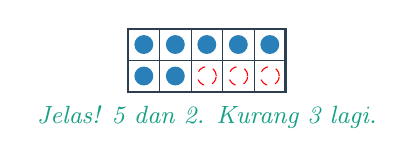
\begin{tikzpicture}[scale=0.4, baseline={([yshift=-.5ex]current bounding box.center)}]
            \draw[mainBlue, thin] (0,0) grid (5,2);
            \draw[mainBlue, thick] (0,0) rectangle (5,2);
            % Fill 7 organized
            \foreach \x in {0.5, 1.5, 2.5, 3.5, 4.5} \fill[dotBlue] (\x, 1.5) circle (0.3);
            \foreach \x in {0.5, 1.5} \fill[dotBlue] (\x, 0.5) circle (0.3);
            % Empty slots highlight
            \foreach \x in {2.5, 3.5, 4.5} \draw[dashed, red] (\x, 0.5) circle (0.3);
            
            % Caption inside tikzpicture
            \node[font=\small\itshape, text=accentTeal] at (2.5, -0.8) {Jelas! 5 dan 2. Kurang 3 lagi.};
        \end{tikzpicture}
    \end{minipage}
\end{tcolorbox}

% --- SECTION 2: ANATOMI ---
\begin{tcolorbox}[title=\textbf{2. ANATOMI \& FILOSOFI DESAIN}, colback=white, colframe=accentTeal, coltitle=white, fonttitle=\bfseries\large]
    \begin{minipage}{0.45\textwidth}
        \centering
        \begin{tikzpicture}[tfPic]
            \DrawFrame{0}{0}
            \node[font=\bfseries\scriptsize, text=mainBlue] at (2.5, 2.3) {BARIS ATAS (5 Kotak)};
            \node[font=\bfseries\scriptsize, text=mainBlue] at (2.5, -0.3) {BARIS BAWAH (5 Kotak)};
            \draw[decorate, decoration={brace, amplitude=5pt}, thick, color=niceOrange] (5.1, 2) -- (5.1, 0) node [midway, right=4pt, align=left, text=niceOrange, font=\bfseries\small] {Total\\10};
        \end{tikzpicture}
    \end{minipage}%
    \hfill
    \begin{minipage}{0.5\textwidth}
        \textbf{Logika Desain 2 x 5:}
        \begin{itemize}[leftmargin=*]
            \item Mengikuti pola jari tangan manusia (5 + 5).
            \item Otak sulit memproses >5 objek acak sekaligus. Ten Frame memecahnya menjadi bagian yang mudah dikelola (\textit{chunking}).
        \end{itemize}
    \end{minipage}
\end{tcolorbox}

% --- SECTION 3: JEMBATAN C-P-A ---
\begin{tcolorbox}[title=\textbf{3. JEMBATAN C-P-A (ALUR BELAJAR)}, colback=softBgA, colframe=niceOrange, coltitle=white, fonttitle=\bfseries\large]
    \centering
    \begin{tikzpicture}[node distance=0.2cm and 0.5cm]
        \node[conceptBox] (concrete) {
            \textbf{A. KONKRET}\\ \textit{"Benda Nyata"}\\
            \vspace{0.1cm}
            \begin{tikzpicture}[scale=0.4, baseline={([yshift=-0.5ex]current bounding box.center)}]
                \fill[dotBlue] (-1.2, 0.5) circle (0.3);
                \fill[dotBlue] (-0.3, 0.9) circle (0.3);
                \fill[dotBlue] (0.6, 0.4) circle (0.3);
                \fill[dotBlue] (1.4, 0.8) circle (0.3);
                \fill[dotBlue] (-0.7, -0.3) circle (0.3);
                \fill[dotBlue] (0.9, -0.5) circle (0.3);
            \end{tikzpicture}
        };
        \node[conceptBox, right=of concrete] (bridge) {
            \textbf{B. JEMBATAN}\\ \textit{"Masuk Frame"}\\
            \vspace{0.1cm}
            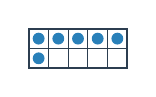
\begin{tikzpicture}[x=0.25cm, y=0.25cm] 
                \draw[mainBlue, thin, step=1] (0,0) grid (5,2);
                \draw[mainBlue, thick] (0,0) rectangle (5,2);
                \foreach \x in {0.5, 1.5, 2.5, 3.5, 4.5} \fill[dotBlue] (\x, 1.5) circle (0.3);
                \foreach \x in {0.5} \fill[dotBlue] (\x, 0.5) circle (0.3);
            \end{tikzpicture}
        };
        \node[conceptBox, right=of bridge] (pictorial) {
            \textbf{C. PIKTORIAL}\\ \textit{"Gambar Mental"}\\
            \vspace{0.1cm}
            \tikz{\node[cloud, cloud puffs=8, draw, fill=gray!10] {\textbf{"6"}};}
        };
        \draw[arrowFlow] (concrete) -- (bridge);
        \draw[arrowFlow] (bridge) -- (pictorial);
    \end{tikzpicture}
\end{tcolorbox}

\begin{center}
    \small \textit{Dikembangkan Berdasarkan Kurikulum Singapore Math \& Prinsip CPA}
\end{center}

\newpage

% =================================================================================
% PART 2: MASTERY & CASE STUDIES
% =================================================================================

% --- REDEFINE TIKZ STYLES FOR PART 2 (More Compact for Case Studies) ---
\tikzset{
    tfPic/.style={x=0.55cm, y=0.55cm, baseline={([yshift=-.5ex]current bounding box.center)}},
    tfGrid/.style={draw=mainBlue, thin, step=1},
    tfBorder/.style={draw=mainBlue, very thick},
    counter/.style={circle, fill=powerBlue, minimum size=0.4cm, inner sep=0pt, drop shadow={opacity=0.3, shadow xshift=1pt, shadow yshift=-1pt}},
    counterRed/.style={circle, fill=alertRed, minimum size=0.4cm, inner sep=0pt, drop shadow={opacity=0.3, shadow xshift=1pt, shadow yshift=-1pt}},
    ghostCounter/.style={circle, draw=alertRed, dashed, thick, minimum size=0.4cm, inner sep=0pt},
    crossOut/.style={cross out, draw=black, very thick, minimum size=0.4cm},
    arrowFlow/.style={->, >={Latex[width=3mm,length=3mm]}, ultra thick, draw=accentTeal}
}

% --- HEADER PART 2 ---
\begin{tcolorbox}[colback=mainBlue, colframe=mainBlue, arc=0mm, boxrule=0pt, top=4mm, bottom=4mm, halign=center]
    {\Huge \bfseries \color{white} TEN FRAME MASTERY} \\
    \vspace{0.1cm}
    {\large \color{accentTeal} \textbf{Analisis Masalah \& Intervensi Visual (Pendekatan Singapore Math)}}
\end{tcolorbox}

\vspace{0.3cm}

% --- INTRO SINGKAT ---
\begin{tcolorbox}[colback=softBgB, colframe=accentTeal, title=\textbf{FILOSOFI PENGGUNAAN}, coltitle=white, fonttitle=\bfseries]
    Bagian ini membedah \textit{learning obstacles} siswa dan bagaimana Ten Frame memfasilitasi transisi dari \textbf{Concrete} (benda nyata) ke \textbf{Abstract} (simbol angka), sesuai prinsip Singapore Math.
\end{tcolorbox}

\vspace{0.3cm}

% --- KASUS 1 ---
\begin{CaseStudyBox}{KASUS 1: "SAYA HARUS HITUNG SATU-SATU DARI AWAL"}
\begin{minipage}{0.3\textwidth}
    \centering
    \begin{tikzpicture}[tfPic]
        \DrawFrame{0}{0}
        % Pattern 7: 5 top, 2 bottom
        \foreach \x in {0.5, 1.5, 2.5, 3.5, 4.5} \node[counter] at (\x, 1.5) {};
        \foreach \x in {0.5, 1.5} \node[counter] at (\x, 0.5) {};
        
        % Visual cue grouping
        \draw[decorate, decoration={brace, mirror, amplitude=3pt}, thick, powerBlue] (0, 1.9) -- (5, 1.9) node[midway, above=2pt, font=\tiny\bfseries] {LIMA (Full)};
        \draw[decorate, decoration={brace, amplitude=3pt}, thick, niceOrange] (0, 0.1) -- (2, 0.1) node[midway, below=2pt, font=\tiny\bfseries] {DUA};
    \end{tikzpicture}
\end{minipage}%
\hfill
\begin{minipage}{0.68\textwidth}
    \begin{itemize}[leftmargin=0.4cm, label={}]
        \item \textbf{\textcolor{alertRed}{Masalah (The Struggle):}} \textit{Counting All}. 
        Siswa melihat 7 benda. Otaknya tidak memproses "7" sebagai kesatuan, melainkan urutan "1, 2, 3, 4, 5, 6, 7". Ini membebani \textit{working memory} dan rentan salah hitung.
        
        \item \textbf{\textcolor{powerBlue}{Kenapa Ten Frame?}} \textit{Structure as Anchor}.
        Ten Frame memaksa pengelompokan (subitizing). Baris atas penuh selalu berarti 5. Siswa tidak perlu menghitung 5 titik itu lagi.
        
        \item \textbf{\textcolor{solGreen}{Solusi Intervensi:}}
        \textbf{"Flash Cards 2 Detik"}. Tunjukkan frame berisi 7 selama 2 detik lalu tutup. 
        \begin{itemize}[label=-, topsep=0pt, itemsep=0pt, font=\small]
            \item Tanya: "Apa yang kamu lihat?"
            \item Jawaban yang diharapkan: "Saya lihat baris atas penuh (5) dan ada 2 di bawah. Jadi 7."
            \item \textit{Goal:} Mengganti "Counting" dengan "Seeing".
        \end{itemize}
    \end{itemize}
\end{minipage}
\end{CaseStudyBox}

\vspace{0.3cm}

% --- KASUS 2 ---
\begin{CaseStudyBox}{KASUS 2: "SAYA LUPA PASANGAN ANGKA 10"}
\begin{minipage}{0.3\textwidth}
    \centering
    \begin{tikzpicture}[tfPic]
        \DrawFrame{0}{0}
        % 8 dots
        \foreach \x in {0.5, 1.5, 2.5, 3.5, 4.5} \node[counter] at (\x, 1.5) {};
        \foreach \x in {0.5, 1.5, 2.5} \node[counter] at (\x, 0.5) {};
        
        % 2 ghosts
        \node[ghostCounter] at (3.5, 0.5) {};
        \node[ghostCounter] at (4.5, 0.5) {};
        
        \draw[->, alertRed, thick] (4.5, -0.2) to[out=-45, in=-90] (5.5, 0.5) node[right, font=\scriptsize\bfseries, align=left] {KOSONG\\JELAS};
    \end{tikzpicture}
\end{minipage}%
\hfill
\begin{minipage}{0.68\textwidth}
    \begin{itemize}[leftmargin=0.4cm, label={}]
        \item \textbf{\textcolor{alertRed}{Masalah (The Struggle):}} \textit{Abstract Memorization}. 
        Siswa menghafal $8+2=10$ seperti menghafal puisi. Jika lupa, mereka kembali menghitung jari dan sering kehabisan jari.
        
        \item \textbf{\textcolor{powerBlue}{Kenapa Ten Frame?}} \textit{Negative Space}.
        Mata manusia sama peka-nya terhadap "isi" dan "kosong". Ten Frame memvisualisasikan "apa yang hilang" (the missing part) sejelas "apa yang ada".
        
        \item \textbf{\textcolor{solGreen}{Solusi Intervensi:}}
        \textbf{"Analogi Kursi Bus"}. 
        \begin{itemize}[label=-, topsep=0pt, itemsep=0pt, font=\small]
            \item Cerita: "Bus kapasitas 10. Sudah naik 8 penumpang (biru)."
            \item Tanya: "Berapa kursi kosong yang terlihat?" (Siswa langsung menunjuk 2 kotak kosong).
            \item Konsep: $10 - 8 = 2$ atau $8 + 2 = 10$ menjadi visual, bukan hafalan.
        \end{itemize}
    \end{itemize}
\end{minipage}
\end{CaseStudyBox}

\vspace{0.3cm}

% --- KASUS 3 ---
\begin{CaseStudyBox}{KASUS 3: "9 + 5 SUSAH, JARI SAYA CUMA 10"}
\begin{minipage}{0.3\textwidth}
    \centering
    \begin{tikzpicture}[tfPic, scale=0.8]
        % Frame 9
        \DrawFrame{0}{2.5}
        \foreach \x in {0.5, 1.5, 2.5, 3.5, 4.5} \node[counter] at (\x, 4) {};
        \foreach \x in {0.5, 1.5, 2.5, 3.5} \node[counter] at (\x, 3) {};
        \node[right, font=\tiny] at (5, 3.5) {9};

        % Frame 5
        \DrawFrame{0}{0}
        \foreach \x in {0.5, 1.5, 2.5, 3.5, 4.5} \node[counterRed] at (\x, 1.5) {};
        \node[right, font=\tiny] at (5, 1) {5};
        
        % The Move
        \draw[->, black, dashed, thick] (0.5, 1.5) to[out=110, in=-90] (4.5, 3);
        \node[draw=black, fill=yellow!20, font=\tiny, align=center, rotate=30] at (3, 2.2) {PINDAH 1};
    \end{tikzpicture}
\end{minipage}%
\hfill
\begin{minipage}{0.68\textwidth}
    \begin{itemize}[leftmargin=0.4cm, label={}]
        \item \textbf{\textcolor{alertRed}{Masalah (The Struggle):}} \textit{Crossing the Ten}. 
        Saat penjumlahan melebihi 10, siswa sering bingung "menyimpan" angka di kepala (\textit{carrying over}). 
        
        \item \textbf{\textcolor{powerBlue}{Kenapa Ten Frame?}} \textit{Decomposition \& Composition}.
        Memungkinkan siswa memanipulasi angka: memecah 5 menjadi (1 + 4) untuk melengkapi 9 menjadi 10.
        
        \item \textbf{\textcolor{solGreen}{Solusi Intervensi:}}
        \textbf{"Make a Ten Strategy"}.
        \begin{itemize}[label=-, topsep=0pt, itemsep=0pt, font=\small]
            \item Instruksi: "9 itu 'rakus', dia ingin jadi 10. Dia minta 1 dari 5."
            \item Aksi: Geser 1 kancing fisik dari frame 5 ke frame 9.
            \item Hasil Visual: Sekarang kita punya \textbf{1 frame penuh (10)} dan \textbf{sisa 4}.
            \item Abstraksi: $9 + 5 \rightarrow 10 + 4 = 14$. Jauh lebih mudah bagi otak.
        \end{itemize}
    \end{itemize}
\end{minipage}
\end{CaseStudyBox}

\vspace{0.3cm}

% --- KASUS 4 ---
\begin{CaseStudyBox}{KASUS 4: "BERAPA LEBIHNYA 7 DARI 4?"}
\begin{minipage}{0.3\textwidth}
    \centering
    \begin{tikzpicture}[tfPic]
        \DrawFrame{0}{0}
        % 7 counters
        \foreach \x in {0.5, 1.5, 2.5, 3.5, 4.5} \node[counter] at (\x, 1.5) {};
        \foreach \x in {0.5, 1.5} \node[counter] at (\x, 0.5) {};
        
        % 4 counters (different color/shape implies comparison)
        % We overlay X to show comparison logic: cancel out matches
        \foreach \x in {0.5, 1.5, 2.5, 3.5} \node[text=white, font=\bfseries] at (\x, 1.5) {=};
        
        \draw[decorate, decoration={brace, amplitude=4pt}, thick, alertRed] (4.1, 1.1) -- (4.9, 1.9) node[midway, right=3pt, font=\tiny, align=left, color=black] {Sisa\\ini};
        \draw[decorate, decoration={brace, amplitude=4pt, mirror}, thick, alertRed] (-0.1, 0.1) -- (2.1, 0.1) node[midway, below=2pt, font=\tiny, color=black] {Sisa ini};
    \end{tikzpicture}
\end{minipage}%
\hfill
\begin{minipage}{0.68\textwidth}
    \begin{itemize}[leftmargin=0.4cm, label={}]
        \item \textbf{\textcolor{alertRed}{Masalah (The Struggle):}} \textit{Comparison Concept}. 
        Siswa bingung bedanya "dikurangi" (take away) dengan "selisih" (difference). Kalimat "Berapa lebih banyak A daripada B?" terdengar abstrak.
        
        \item \textbf{\textcolor{powerBlue}{Kenapa Ten Frame?}} \textit{Linear Alignment}.
        Grid memastikan setiap item punya posisi pasti. Kita bisa melakukan korespondensi satu-satu (matching) secara visual.
        
        \item \textbf{\textcolor{solGreen}{Solusi Intervensi:}}
        \textbf{"Pasang-Pasangkan"}. 
        \begin{itemize}[label=-, topsep=0pt, itemsep=0pt, font=\small]
            \item Masukkan 7 kancing biru. Masukkan 4 kancing merah di atasnya (tumpuk) atau di frame bawah.
            \item "Ayo kita jodohkan." 4 punya pasangan, sisanya (3) jomblo/sendiri.
            \item Bagian yang "menggantung" atau tidak punya pasangan itulah bedanya.
        \end{itemize}
    \end{itemize}
\end{minipage}
\end{CaseStudyBox}

\newpage

% --- KASUS 5 ---
\begin{CaseStudyBox}{KASUS 5: "13 ITU APA? SATU DAN TIGA?"}
\begin{minipage}{0.3\textwidth}
    \centering
    \begin{tikzpicture}[tfPic, scale=0.8]
        % Frame 10 (Full)
        \DrawFrame{0}{2.5}
        \foreach \x in {0.5, 1.5, 2.5, 3.5, 4.5} {
            \node[counter] at (\x, 4) {};
            \node[counter] at (\x, 3) {};
        }
        \node[font=\bfseries\tiny, color=mainBlue, anchor=west] at (5.1, 3.5) {1 Puluhan};

        % Frame 3 (Part)
        \DrawFrame{0}{0}
        \foreach \x in {0.5, 1.5, 2.5} \node[counterRed] at (\x, 1.5) {};
        \node[font=\bfseries\tiny, color=alertRed, anchor=west] at (5.1, 1) {3 Satuan};
        
        \node[font=\bfseries\Large] at (2.5, -0.8) {10 + 3 = 13};
    \end{tikzpicture}
\end{minipage}%
\hfill
\begin{minipage}{0.68\textwidth}
    \begin{itemize}[leftmargin=0.4cm, label={}]
        \item \textbf{\textcolor{alertRed}{Masalah (The Struggle):}} \textit{Place Value Confusion}. 
        Siswa sering melihat angka "13" sebagai digit "1" dan "3". Mereka tidak sadar bahwa "1" itu bernilai 10.
        
        \item \textbf{\textcolor{powerBlue}{Kenapa Ten Frame?}} \textit{Unitizing Ten}.
        Visual ini membuktikan bahwa 1 frame penuh adalah "satu kelompok sepuluh". 13 tidak pernah terlihat sebagai 1 dan 3 terpisah, tapi "Satu frame penuh dan tiga sisa".
        
        \item \textbf{\textcolor{solGreen}{Solusi Intervensi:}}
        \textbf{"Say Ten Counting"}.
        \begin{itemize}[label=-, topsep=0pt, itemsep=0pt, font=\small]
            \item Jangan hanya sebut "tiga belas". Gunakan bahasa matematika: "Satu puluhan tiga satuan" (One ten three).
            \item Minta siswa membuat semua angka belasan dengan 2 frame. Yang atas HARUS penuh dulu.
        \end{itemize}
    \end{itemize}
\end{minipage}
\end{CaseStudyBox}

\vspace{0.3cm}

% --- KASUS 6 ---
\begin{CaseStudyBox}{KASUS 6: "LUPA MANA GANJIL MANA GENAP"}
\begin{minipage}{0.3\textwidth}
    \centering
    \begin{tikzpicture}[tfPic]
        \DrawFrame{0}{0}
        % 7 Counters
        \foreach \x in {0.5, 1.5, 2.5} {
            \node[counter] at (\x, 1.5) {}; 
            \node[counter] at (\x, 0.5) {}; 
            \draw[thick, green!60!black] (\x, 1.5) -- (\x, 0.5); % Pairing lines
        }
        % The odd one
        \node[counter] at (3.5, 1.5) {};
        
        \draw[->, alertRed, thick] (3.5, 1.5) -- (3.5, 2.3) node[above, font=\tiny\bfseries] {SENDIRI!};
        \node[font=\bfseries] at (2.5, -0.6) {7 (Ganjil)};
    \end{tikzpicture}
\end{minipage}%
\hfill
\begin{minipage}{0.68\textwidth}
    \begin{itemize}[leftmargin=0.4cm, label={}]
        \item \textbf{\textcolor{alertRed}{Masalah (The Struggle):}} \textit{Rote Memorization}. 
        Siswa menghafal "1, 3, 5 itu ganjil" tanpa paham kenapa. Sering tertukar saat angka membesar.
        
        \item \textbf{\textcolor{powerBlue}{Kenapa Ten Frame?}} \textit{Pairing Structure}.
        Ten Frame disusun 2 baris (pair-wise). Sifat genap (berpasangan) dan ganjil (ada sisa) terlihat instan tanpa hitung bagi.
        
        \item \textbf{\textcolor{solGreen}{Solusi Intervensi:}}
        \textbf{"Temukan Temannya"}.
        \begin{itemize}[label=-, topsep=0pt, itemsep=0pt, font=\small]
            \item Masukkan kancing ke frame secara berpasangan (atas-bawah, atas-bawah).
            \item Jika di akhir ada kancing yang tidak punya teman di bawahnya $\rightarrow$ GANJIL (Odd).
            \item Jika semua rapi berpasangan $\rightarrow$ GENAP (Even).
        \end{itemize}
    \end{itemize}
\end{minipage}
\end{CaseStudyBox}

\vspace{0.3cm}

% --- KASUS 7 ---
\begin{CaseStudyBox}{KASUS 7: "14 - 6 ITU SULIT SEKALI"}
\begin{minipage}{0.3\textwidth}
    \centering
    \begin{tikzpicture}[tfPic, scale=0.8]
        % Frame 10 (Full) with 2 crossed out
        \DrawFrame{0}{2.5}
        \foreach \x in {0.5, 1.5, 2.5} {
            \node[counter] at (\x, 4) {};
            \node[counter] at (\x, 3) {};
        }
        \foreach \x in {3.5, 4.5} {
            \node[counter] at (\x, 4) {};
            \node[counter] at (\x, 3) {};
        }
        % Cross out 2 from top frame
        \node[crossOut] at (4.5, 3) {};
        \node[crossOut] at (3.5, 3) {};
        \node[font=\tiny, color=alertRed] at (4, 4.6) {-2};

        % Frame 4 (Part) ALL crossed out
        \DrawFrame{0}{0}
        \foreach \x in {0.5, 1.5, 2.5, 3.5} {
            \node[counterRed] at (\x, 1.5) {};
            \node[crossOut] at (\x, 1.5) {};
        }
        \node[font=\tiny, color=alertRed] at (2, -0.6) {-4 (Habiskan dulu)};
    \end{tikzpicture}
\end{minipage}%
\hfill
\begin{minipage}{0.68\textwidth}
    \begin{itemize}[leftmargin=0.4cm, label={}]
        \item \textbf{\textcolor{alertRed}{Masalah (The Struggle):}} \textit{Hard Subtraction}. 
        $14 - 6$. Siswa menghitung mundur 6 kali pakai jari, sering selip hitung.
        
        \item \textbf{\textcolor{powerBlue}{Kenapa Ten Frame?}} \textit{Part-Part-Whole}.
        Strategi visual: Buang dulu sisa satuannya (4), baru ambil sisanya dari puluhan utuh.
        
        \item \textbf{\textcolor{solGreen}{Solusi Intervensi:}}
        \textbf{"Habiskan Ekornya Dulu"}.
        \begin{itemize}[label=-, topsep=0pt, itemsep=0pt, font=\small]
            \item Soal: $14 - 6$.
            \item Langkah 1: "Kita punya 14 (10 dan 4). Buang dulu 4 yang di bawah." (Sisa mau buang 2 lagi).
            \item Langkah 2: "Ambil 2 dari frame penuh."
            \item Siswa melihat sisa 8 di frame atas. Visual $10 - 2 = 8$ jauh lebih mudah.
        \end{itemize}
    \end{itemize}
\end{minipage}
\end{CaseStudyBox}

\end{document}
